% !TeX root = main.tex

\section{Use cases}
The PRS has five use cases which describes the life-cycle from initialisation to revocation of a petrol card. Figure 1 depicts the PRS life-cycle. 

\begin{itemize}
\item Initialisation of the petrol card with the issuer terminal (IT):\\
During the personalisation phase the petrol card will be initialised with key material, a card identification number (both provided by back-end) and the current petrol balance will be set to zero. 
%A process (out of scope) needs to be in place to e.g. register the petrol card to the car owner. 

\item Charging the petrol card at the charging terminal (CT): \\
The charging terminal will receive a monthly update for the petrol allowance from the back-end, which determines the amount of petrol that will be written to all petrol cards. For each presented petrol card a validation is needed if the petrol card is still valid, afterwards the card owner can charge the full monthly petrol allowance to his petrol card balance. Sub-charges of the petrol allowance are not possible. The updated balance will be immediately available for use. 

\item Getting petrol at the petrol terminal (PT):\\
At the petrol terminal the card owner presents his petrol card. The card owner is able to see his current petrol allowance, after choosing the type of petrol and the amount of petrol he wishes to buy, the PT will remove the chosen petrol balance from the petrol card. %After the transaction has been completed the updated balance will be written back to the petrol card. 

\item End-of-life: \\
Once a card reaches end-of-life (EOL), it has to be blocked and possibly decommissioned. After 5 years petrol cards will automatically be blocked.

\item Stolen Card: \\
If a card is stolen or lost, all key material and certificates needs to be revoked. All petrol and charging terminals will receive an updated revocation list during the night. 

%The image shows the life-cycle of the PRS. 
\begin{figure}[!ht]
  \centering
    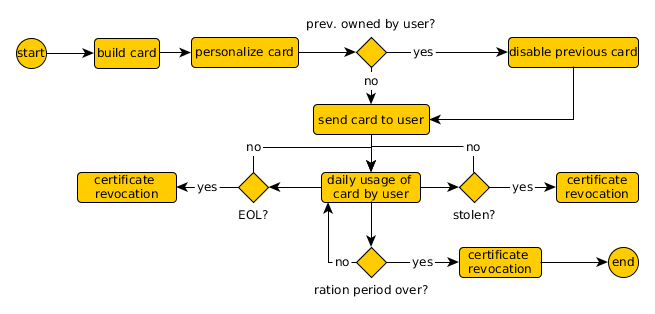
\includegraphics[width=0.8\textwidth]{lifecycle}
      \caption{The life-cycle of a petrol card in the PRS.}

\end{figure}

\end{itemize}